\chapter{The Spatial Compiler}
\label{compiler}

Now that we have defined our input representation (parallel patterns) and given
an overview of our Spatial hardware abstraction, we next describe the lowering
process and the details of the Spatial compiler. Since Spatial is designed to
to target reconfigurable architectures like FPGAs, there are a
number of analyses and optimizations that differ from standard software compilers.
The compiler's key passes are summarized in Figure~\ref{fig:spatial-diag} and
described in this chapter.

\begin{figure*}
\centering
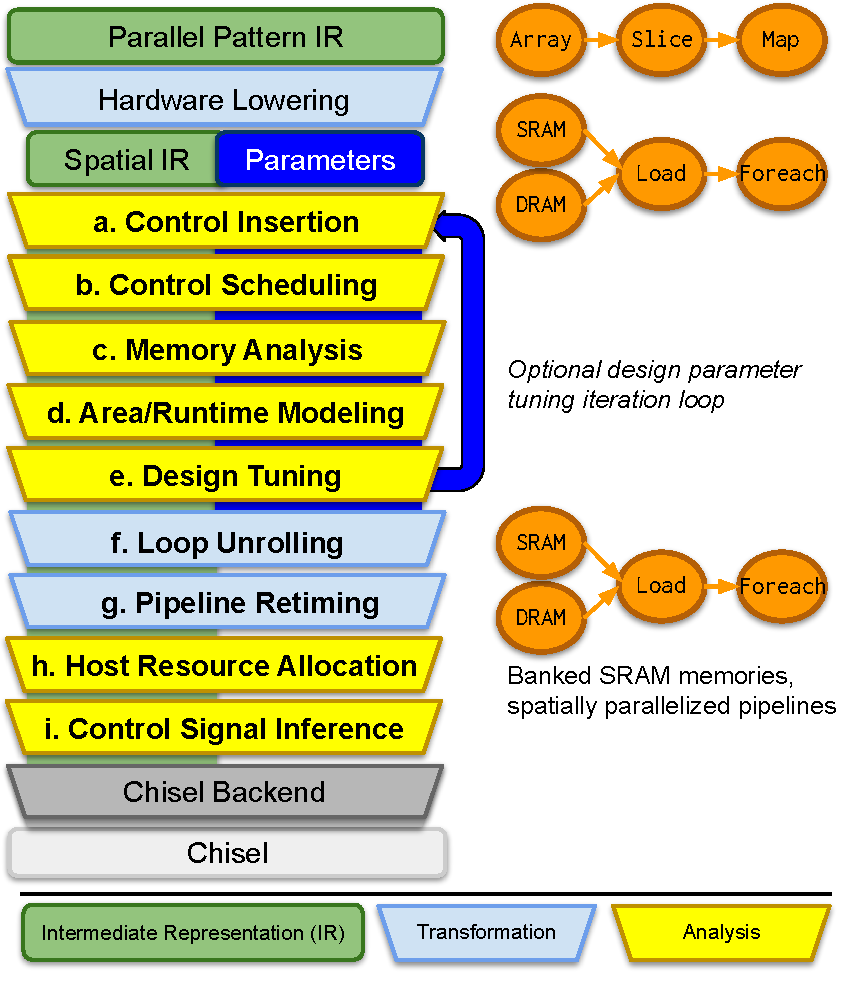
\includegraphics[width=0.8\textwidth]{5-compiler/figs/spatial-diag}
\caption{\label{fig:spatial-diag}Block diagram of the Spatial compiler.
This compiler optimizes the Spatial hardware IR for a selected FPGA target
and generates synthesizable Chisel RTL.}
\end{figure*}

The Spatial compiler provides translations from applications or IR
in the Spatial abstraction to synthesizable hardware descriptions in Chisel RTL~\cite{chisel}.
The input to Spatial can be either in the form of the accompanying Spatial language for ``power'' users,
or in-memory tiled parallel patterns when compiling from higher level DSLs.
The generated Chisel RTL is then compiled by the third party Chisel compiler and used
to generate Verilog, which can in turn be synthesized on an FPGA target using vendor tools.
Spatial also generates host code in C++ for FPGA runtime administration and data management.



\section{Intermediate Representation}

Spatial programs are internally represented in the compiler as a hierarchical dataflow graph (DFG).
Nodes in this graph represent control structures, data operations, and memory allocations, while edges represent data and effect dependencies.
Nesting of controllers directly translates to the hierarchy in the intermediate representation.
Design parameters are kept as graph metadata, such that they can be independently updated without changing the graph itself.

\newsavebox{\gemm}
\begin{lrbox}{\gemm}
\begin{lstlisting}[language=Spatial,linewidth=0.4\textwidth]
// Load data from files
val a = loadMatrix[Float](args(0))
val b = loadMatrix[Float](args(1))

// Allocate space on accelerator DRAM
val A = DRAM[Float](a.rows,a.cols)
val B = DRAM[Float](b.rows,b.cols)
val C = DRAM[Float](a.rows,b.cols)

// Create explicit design parameters
val M = 128 (64, 1024)  // Tile size - rows
val N = 128 (64, 1024)  // Tile size - cols
val P = 128 (64, 1024)  // Tile size - common
val PAR_K  = 2 (1, 8)   // Unroll factor of k
val PAR_J  = 2 (1, 16)  // Unroll factor of j

// Transfer data to accelerator DRAM
sendMatrix(A, a)
sendMatrix(B, b)

// Specify the accelerator design
Accel {
  // Produce C in M x N tiles
  Foreach(A.rows by M, B.cols by N){
    (ii,jj) =>
    val tileC = SRAM[Float](M, N)
    // Combine intermediates (outer)
    MemReduce(tileC)(A.cols by P){ kk =>
      // Allocate on-chip scratchpads
      val tileA = SRAM[Float](M, P)
      val tileB = SRAM[Float](P, N)
      val accum = SRAM[Float](M, N)

      // Load tiles of A and B from DRAM
      tileA load A(ii::ii+M, kk::kk+P)
      tileB load B(kk::kk+P, jj::jj+N)

      // Combine intermediates (across P)
      MemReduce(accum)(P par PAR_K){ k =>
        val partC = SRAM[Float](M, N)
        Foreach(M by 1, N par PAR_J){ (i,j) =>
          partC(i,j) = tileA(i,k) * tileB(k,j)
        }
        partC
      // Combine with element-wise add
      }{(a,b) => a + b }
    }{(a,b) => a + b }

    // Store the tile of C to DRAM
    C(ii::ii+M, jj::jj+N) store tileC
  }
}
// Save the result to another file
saveMatrix(args(2), getMatrix(C))
\end{lstlisting}
\end{lrbox}

\begin{figure}
\begin{tabular}{cm{0.4\textwidth}m{0.6\textwidth}}
{\hspace{10pt}\usebox{\gemm}} &
{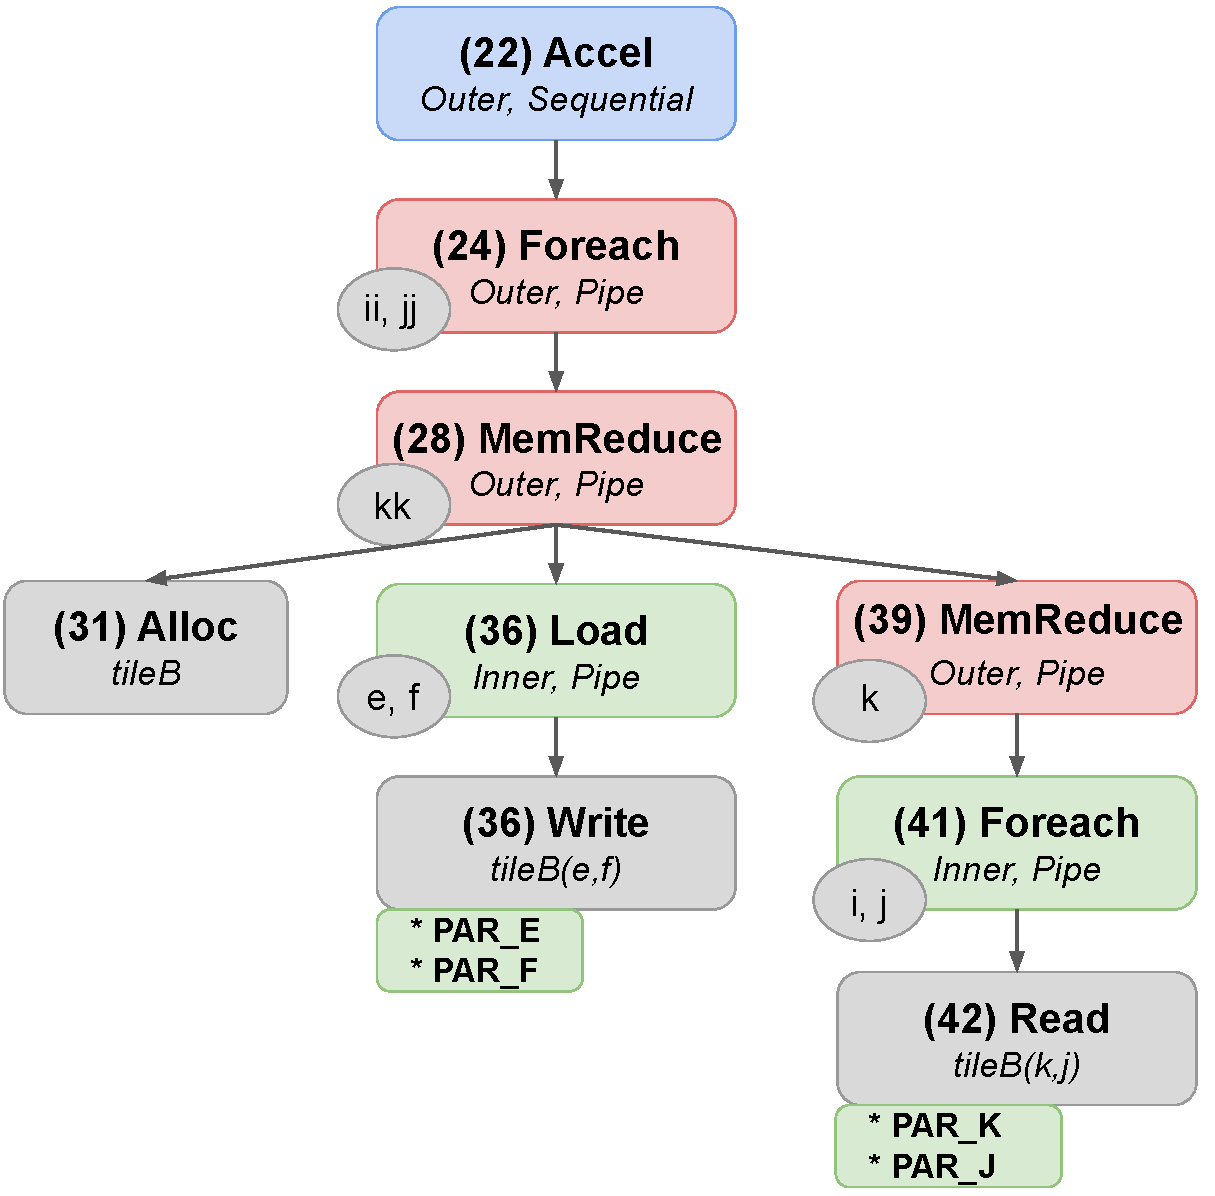
\includegraphics[width=0.55\textwidth]{5-compiler/figs/ctrltree.pdf}} \\
{\parbox{0.4\textwidth}{\centering{a. Spatial implementation. }}} &
{\parbox{0.6\textwidth}{\centering{b. Control/access tree for \texttt{\small{tileB}}.}}}
\end{tabular} %% end resizebox
\caption{Matrix multiplication ($C$~=~$A~\cdot~B$) implemented in Spatial and corresponding control/access tree IR. Control nodes are annotated with their control level, schedule, and loop iterator name. Outer sequential nodes are blue, outer pipeline nodes are red, and inner pipelined control nodes are green. Memory access nodes (gray) are annotated with their parallelization factor.}
\label{fig:matmult}
\end{figure}


When discussing DFG transformations and optimizations, it is often useful to think about the graph as a controller/access tree. Figure~\ref{fig:matmult} shows an example of one such controller tree for the memory {\texttt{\small{tileB}} in the Spatial code example of matrix multiplication. Note that transfers between on-chip and off-chip memory each expand to a control node which linearly accesses the on-chip memory, in this case by iterators \texttt{e} and \texttt{f}.
This tree abstracts away most primitive operations, leaving only relevant controller hierarchy and the memory
accesses for a specific memory.

Within the acceleratable subset of Spatial, nodes are formally separated into three categories:
control nodes, memory allocation nodes, and primitive nodes.
Control nodes represent state machine structures like \texttt{\small{Foreach}} and \texttt{\small{Reduce}} described in Chapter~\ref{controls}.
Primitive nodes are operations which may consume, but never produce, control signals, including on-chip memory accesses.
Primitive nodes are further broken down into ``physical'' operations requiring resources and ``ephemeral'' operations which are only used for bookkeeping purposes in the compiler. For example, bit selects and grouping of words into structs require no hardware resources but are used to track necessary wires in the generated code.



% The nodes that compose the IR of Spatial provide the handles necessary to do a range of
% hardware optimizations that are specific to spatial architectures.  The combination of
% metadata associated with each node and the hierarchical structure AST that exposes relationships
% between primitives and control structures make it easy to do optimizations on the scheduling of
% controllers, buffering, banking, and duplication of memory elements, and comprehensive DSE over
% the provided parameter space with low latency.
% \subsection{DRAM Request Consolidation}
% In memory-bound applications, the only way to improve performance is to make better use
% of the available bandwidth.  It is well known that memory bandwidth asymptotically approaches the DRAM's peak bandwidth \todo{is this true?}
% as the size of each request increases.  This is because of how DRAM pays a penalty for activating and retiring
% lines of memory cells, and can return more data quickly when consecutive bursts are requested with the same command.

% Unfortunately, there are many applications where the programmer may opt to create logical tensors with
% relatively small leading dimensions and attempt to load multi-dimensional portions of the structure into on-chip SRAM
% without awareness of how this may thrash the DRAM's controllers in an inefficient way.  For example,
% the programmer may want to solve a multi-objective gradient descent problem that has many training points and very
% few objectives, hence creating a tall and skinny Y matrix.

% The compiler is able to recognize when the application will be sending out multiple requests to DRAM with
% consecutive addresses, and rewrite the controller to consolidate these into fewer, longer burst commands.
% This means that the user will get fully optimized DRAM requests and physical hardware without needing
% to rethink or change the semantics of the source code.

\section{Control Insertion}
Spatial requires that control nodes do not contain both physical primitive nodes and other control nodes.
While not strictly necessary for correctness, this transformation simplifies
other analysis passes by providing the contract that every memory access occurs
in an inner controller, thus making the hierarchy of control signals from outer
controllers to inner accesses more straightforward.
This requirement is satisfied by a DFG transformation which inserts \texttt{\small{DummyPipe}} control nodes around primitive logic in control bodies which also contain control nodes. The \texttt{\small{DummyPipe}} node is a bookkeeping control structure which is logically equivalent to a loop with exactly one iteration.
Thereafter, control nodes with primitive nodes are called ``inner'' control nodes, while controllers which contain other nested controllers are called ``outer'' nodes.

% For example, Figure~\ref{fig:matmult} contains some of these nodes. The Foreach in line 32 is an ``outer'' controller, which contains a memory allocation node for tileC
% (line 33) and another control node, \texttt{\small{MemReduce}} in line 38.  The \texttt{\small{Foreach}} in line 51 is an ``inner'' controller, as it contains
% only primitive nodes generated by the SRAM reads, multiplication, and SRAM store inlined on line 52.


\section{Controller Scheduling}
\label{scheduling}
After controller insertion, the compiler will then schedule the operations within each controller. Currently, Spatial assumes a fixed clock rate across all parts of the
hardware accelerator design, and pipelines all primitive operations to maximize
likelihood of fitting this clock rate.
By default, the compiler will always attempt to pipeline loops regardless of nesting level.
The behavior of the compiler's scheduler can be overridden by the user using the directives listed in Table~\ref{t:syntaxTable}b.

Inner pipeline schedules are based on their initiation interval in terms of clock cycles.
The initiation interval calculated here is for a single loop iteration, independent of parallelization factor. Unless forced by the user, Spatial does not parallelize loops with an initiation
interval greater than 1, as this will usually result in behavior inconsistent with
sequential execution.
The compiler first collects resource initiation intervals for each primitive node in the given controller based on an internal, target-dependent lookup table.
Most primitive operations are pipelined for a resource initiation interval of 1.
The compiler then calculates all loop carried dependencies within the pipeline based on the dataflow graph.
For non-addressable memories, the total initiation interval is the maximum of path lengths between all dependent reads and the writes.
For addressable memories, the path length of loop carried dependencies is also multiplied by the difference in write and read addresses.
If the addresses are loop-independent, the initiation interval is the path length if they may be equal, and 1 if they are provably not equal. If the distance between the addresses cannot be determined statically, the initiation interval is infinite, meaning the loop must be run sequentially.
The total initiation interval is defined as the maximum of the initiation intervals of all loop carried dependencies and all resource initiation intervals.

The compiler also attempts to pipeline the bodies of outer control nodes in a similar manner, but computes dataflow scheduling in terms of inner control nodes and number of stages rather than primitive nodes and cycles. For example, the outer \texttt{\small{MemReduce}} in line 28 of Figure~\ref{fig:matmult} contains 4 sub-controllers: the load into \texttt{\small{tileA}} (line 35), the load into \texttt{\small{tileB}} (36), the inner \texttt{\small{MemReduce}} (39), and a reduction stage combining intermediate tiles (47). Based on data dependencies, the compiler infers that the two loads can be run in parallel, followed by the inner \texttt{\small{MemReduce}} and the tile reduction. From the information provided
from the higher level compiler or data dependency analysis, it can also determine
that multiple iterations of this outer loop can be pipelined through these stages.

\subsection{Memory Analysis}
\label{memopts}

\begin{figure}
\centering
\hspace{5pt}
\begin{tabular}{l}
\hline\hline
% function ReachingWrites:
%   input: $I_w$ $\rightarrow$ set of sets of writes
%   input: $I_r$ $\rightarrow$ set of sets of reads
%   $I'_w$ = $\emptyset$
%   $R$ = Flatten($I_r$)
%   for all $W$ in $I_w$:
%     $W'$ = {$w~\forall~w \in W$ s.t.
%             $\exists~r \in R$ s.t. MayPrecede($w$,$r$) $\vee~w \cap r \neq \emptyset$}
%     if $W' \neq \emptyset$: add $W'$ to $I'_w$
%   return $I_w'$
% end function

{\begin{lstlisting}[language=Pseudo,linewidth=0.98\columnwidth, mathescape=true]
function GroupAccesses:
   input: $A$ $\rightarrow$ set of reads or writes to $m$

   $G$ = $\emptyset$ set of sets of compatible accesses

   for all accesses $a$ in $A$:
      for all sets of accesses $g$ in $G$:
       if IComp($a$, $a'$) for all $a'$ in $g$ then
          add $a$ to $g$
          break
       else add {$a$} to $G$

   return $G$
end function

function ConfigureMemory:
   input: $A_r$ $\rightarrow$ set of reads of $m$
   input: $A_w$ $\rightarrow$ set of writes to $m$

   $G_r$ = GroupAccesses($A_r$)
   $G_w$ = GroupAccesses($A_w$)

   $I$ = $\emptyset$ set of memory instances

   for all read sets $R$ in $G_r$:
      $I_r$ = {$R$}
      $I_w$ = ReachingWrites($G_w$, $I_r$)
      $i$ = BankAndBuffer($I_r$, $I_w$)
      for each $inst$ in $I$:
         $I'_r$ = ReadSets[$inst$] + $R$
         $I'_w$ = ReachingWrites($G_w$, $I'_r$)
         if OComp($A_1$,$A_2$) $\forall A_1 \neq A_2 \in (G_w \cup I'_r)$ then:
            $i'$ = BankAndBuffer($I'_r$, $I'_w$)
            if Cost($i'$) < Cost($i$) + Cost($inst$) then:
               remove $inst$ from $I$
               add $i'$ to $I$
               break

      if $i$ has not been merged then add $i$ to $I$

   return I
end function
\end{lstlisting}}\\
\hline
\end{tabular}
\caption{Banking and buffering algorithm for calculating instances of on-chip memory $m$.}
\label{fig:bank_alg}
\end{figure}

Loop parallelization only serves to improve performance if there is sufficient on-chip bandwidth to feed the duplicated computation.
Spatial's memory analysis banks and buffers on-chip memories to maximize this available on-chip read and write bandwidth.
Memory banking, also called data partitioning, is the process of dividing a memory's address space across multiple physical instances in order to create
additional ports for concurrent accesses within the same controller.
Partitioning is possible when the access patterns are statically predictable and guaranteed to never conflict access the same port/bank.
While a single port can be time multiplexed, this entirely negates the benefits of parallelization by increasing the whole pipeline's required initiation interval.
Note that while banking can trivially be achieved by memory duplication, Spatial aims to also minimize the total amount of memory resources.

Spatial leverages the memory partitioning strategy based on conflict polytope emptiness testing described by Wang et. al.~\cite{Wang_banking}. We extend this strategy by accounting for random access patterns and memory accesses across nested loops. Random accesses are modeled as additional dimensions in the conflict polytope as if they were additional loop iterators. Spatial minimizes the number of random access symbols used in this way by identifying affine combinations of random values. For example, an access to a memory at address $x$ and $x+1$ only requires one random variable, $x$, as the second is a predictable, affine function of the first.
Spatial also supports banking per dimension to account for cases where only some dimensions are accessed predictably.

Non-addressed memories like \texttt{\small{FIFOs}} and \texttt{\small{FILOs}} are modeled as addressed memories.
Each access to these memory types is represented as a linear access of all loop iterators around the memory access relative to the memory's definition. Spatial forbids parallelization of outer loops around non-addressed accesses, as this violates the guarantee of equivalent behavior to sequential execution.

To handle multiple pipelined accesses across stages within an outer loop, Spatial also automatically buffers on-chip memories.
Buffering creates multiple copies of the
same memory for maintaining versions of the data across overlapped loop iterations.
Without this optimization, pipeline parallel accesses to the same memory across different stages of a coarse-grain pipeline would not be able to run concurrently.
See Appendix~\ref{banking-appendix} for details on how both banking and buffering are computed.


For example, as shown in Figure~\ref{fig:controlTree}, \texttt{\small{tileB}} has two parallelized accesses, the load on line 42 and the read on line 48. If all (implicit and explicit) parallelization factors are set to 2, this corresponds to 4 accesses per loop. Spatial then builds the access polytope corresponding to all accesses in each loop, and determines the banking strategy that works for both loops. In this example, this means the SRAM will be banked such that each element within a 2x2 square will reside
in a different physical bank to allow fully parallel access. If the \texttt{\small{MemReduce}} on line 34 is pipelined, \texttt{\small{tileB}} will be double buffered to protect the reads (line 48) in one iteration of the outer loop
from the writes (line 42) in the next iteration.

Figure~\ref{fig:bank_alg} gives pseudocode for Spatial's algorithm to bank and buffer accesses to a given memory \emph{m} across loop nests. For each access $a$ to $m$, we first define an iteration domain $D$ for that access. This domain is the multi-dimensional space of possible values of all loop iterators for all loops which contain $a$ but which do not contain $m$.

We then group read and write accesses on $m$ into ``compatible'' sets which occur in parallel to the same physical port but which can be banked together (lines 1 -- 14).
Two accesses $a_1$ and $a_2$ within iteration domains $D_1$ and $D_2$
are banking compatible ($IComp$) if
\[ IComp(a_1,a_2) = \nexists~\vec{i} \in (D_1 \cup D_2) ~s.t.~a_1(\vec{i}) = r_2(\vec{i}) \]
where $a(i)$ is the multi-dimensional address corresponding to access $a$ for some vector of iterator values $i$.
This check can be implemented using a polytope emptiness test.

After grouping, each group could be directly mapped to a coherent ``instance'', or copy, of $m$.
However, this approach would typically use more resources than required. To minimize the total number of memory instances, we next greedily merge groups together (lines 25 -- 39). Merging is done when the cost of a merged instance is less than the cost of adding a separate, coherent instance for that group.
Two sets of accesses $A_1$ and $A_2$ allow merging ($OComp$) if
\[ OComp(A_1, A_2) = \nexists~ (a_1 \in A_1, a_2 \in A_2) ~s.t. \]
\[  LCA(a_1, a_2) \in Parallel \cup (Pipe \cap Inner) \]
where \emph{Parallel}, \emph{Pipe}, and \emph{Inner} are the set of Parallel, pipelined, and inner controllers in the program, respectively.
If this condition holds, all accesses between the two instances either occur sequentially or occur as part of a coarse-grain pipeline. Sequential accesses can be time multiplexed, while pipelined accesses are buffered.

\emph{ReachingWrites} returns all writes in each set which may be visible to any read in the given sets of reads. Visibility is possible if the write may be executed before the read and may have an overlapping address space.

The \emph{BankAndBuffer} function produces a single memory instance from memory reads and writes.
Here, each set of accesses is a set of parallel reads or writes to a single port of the memory instance.
Accesses in different sets are guaranteed not to occur to the same port at the same time.
Therefore, a common banking strategy is found which has no bank conflicts for any set of accesses.
This banking strategy is found using iterative polytope emptiness testing as described by Wang et. al.~\cite{Wang_banking}.
A separate emptiness test is run for each set of parallel accesses for each proposed strategy.

The required buffer depth \emph{d} for a pair of accesses $a_1$ and $a_2$ to $m$ is computed as
\[
d(a_1, a_2) = \left\{\begin{matrix} 1 & LCA(a_1, a_2) \in Seq \cup Stream \\ dist(a_1,a_2) & LCA(a_1,a_2) \in Pipe \end{matrix}\right.
\]
where \emph{dist} is the minimum of the depth of the LCA and the dataflow distance of the two direct children of the LCA which contain $a_1$ and $a_2$. \emph{Seq}, \emph{Stream}, and \emph{Pipe} are the set of sequential, streaming, and pipelined controllers, respectively. Buffering addressable memories across streaming accesses is currently unsupported.
The depth of a set of reads $R$ and writes $W$ is then
\[ Depth(R,W) = max\{ d(w,a)~\forall ~(w,a) \in W \times (W\cup R) \} \]

The port of each access within a buffer is determined from the relative distances between all buffered accesses.
Spatial requires that no more than one coarse-grained controller or streaming controller is part of a merged instance.
The final output of the greedy search is a set of required physical memory instances for memory \emph{m}.

\section{Area and Runtime Modeling}
\label{sec:modeling}
In this section, we describe our area and runtime modeling methodology. Our models account for the various
design parameters for each Spatial node, as well as optimizations done by low-level logic
synthesis tools in order to accurately estimate resource usage.

\subsection{Modeling Considerations}
\label{ss:modeling-con}
The resource requirements of a given application implemented on an
FPGA depend both on the target device and on the toolchain.
Heterogeneity in the FPGA fabric, use of FPGA resources for routing,
and other low-level optimizations performed by logic synthesis tools often have
a significant impact on the total resource consumption of a design.
Since these factors reflect the physical layout of computation on the device
after placement and routing, they are not captured directly in the application's dataflow graph.
We identify and account for the following factors:

\paragraph{LUT and register packing} Basic compute units in FPGAs are typically composed of a lookup table (LUT), and a small number of single bit multiplexers, registers, and full adders.
  Modern FPGA LUTs support up to 8-input binary functions but are often implemented using a pair of smaller LUTs~\cite{stratixv,virtex7}.
  When these LUTs can be configured and used independently, vendor placement tools attempt to ``pack'' multiple small functions into a single 8-input unit.
  LUT packing can have a significant impact on design resource requirements.
  In our experiments, we are able to pack about 80\% of the functions in each design in pairs, decreasing the number of used LUTs by about 40\%.

\paragraph{Routing Resources} Logic synthesis tools require a significant amount of resources to establish static routing connections
between two design points (e.g., a multiplier and a block RAM) which fit in the path's clock period. While FPGAs have dedicated routing resources,
logic synthesis tools may have the option to use LUTs for routing. These LUTs may then be unavailable to be used for ``real'' compute.
In our designs, ``route-through'' LUTs typically account for about 10\% of the total number of used LUTs.


\paragraph{Logic duplication} Logic synthesis tools often duplicate resources such as block RAMs
and registers to avoid routing congestion and to decrease fan out. While duplicated registers typically
encompass around 5\% of the total number of registers required in our designs, we found that block RAM
duplication can increase RAM utilization by 10 to 100\%, depending on the complexity of the design.


\paragraph{Unavailable resources} FPGA resources are typically organized in a hierarchy, such as Altera's Logic Array Block structure (10 LUTs)
and Xilinx's Slice structure (4 LUTs). Such organizations impose mapping constraints which can lead to
resources that are rendered unusable. In our experiments, the number of unusable LUTs made up only about 4\% of the design's total LUT usage.

\subsection{Methodology}
In order to model runtime and resource requirements of Spatial designs, we first need an estimate of the area requirements and
propagation delay of every Spatial node. Area requirements include the number of digital signal processing
units (DSPs), device block RAMs, LUTs, and registers that each template requires. To facilitate LUT packing estimation,
we split template LUT resource requirements into the number of ``packable'' and ``unpackable'' LUTs required.
%For templates with documented implementations such as floating point operations \cite{fp-altera}, we gather resource and cycle data in part by summarizing IP core documentation. However, these user manuals typically do not give resource usage breakdowns at the binary function level.
We obtain characterization data by synthesizing multiple instances of each template instantiated for combinations of its parameters, including parallelization factor and control schedule.
Using this data, we create analytical models of each Spatial nodes's resource requirements and cycle counts for
a predefined fabric clock. The area and cycle count of controller templates are modeled as functions of the latencies of the nodes contained within them.
The total cycle count for a coarse-grain pipelined controller, for example,
is modeled using the recursive function
\begin{displaymath}
(N-1)\max(cycles(n) | n \in nodes) + \sum_{n \in nodes} cycles(n)
\end{displaymath}
where \emph{N} is the number of iterations of the controller and \emph{nodes} is the
longest chain of dependencies within the set of children
controllers contained in the coarse-grain pipelined controller.

Most templates require about six synthesized designs to characterize their resource and area usage as a function of their parameters. Note that these models include estimates of off-chip memory access latency as a function of the
number and length of memory commands, as well as contention due to competing accessors. Since template models are application-independent, each needs only be characterized once for a given target device and logic synthesis toolchain. The synthesis times required to model templates can therefore be amortized over many applications.

Using these models, we run a pair of analysis passes over the application's intermediate representation to estimate design cycle counts and area requirements.

\subsubsection{Cycle Count Estimation}
In the first analysis pass, we estimate the total runtime of the design on the FPGA.
Since the Spatial intermediate representation is hierarchical in nature, this pass is done recursively.
The total runtime of coarse-grained pipelines and sequential controllers is calculated first by determining
the runtime of all controller nodes contained within them. The total propagation delay of a single
iteration of a \emph{Pipe} is the length of the body's critical path, calculated using a depth first
search of the body's subgraph and the propagation delay of all primitive nodes within the graph.
Input dataset sizes, given as user annotations in the high-level program, are used by the analysis pass
along with tiling factors to determine the iteration counts for each controller template.
Iteration counts are then used to calculate the total runtime of the respective controller nodes.


\subsubsection{Area Estimation}
Since the FPGA resource utilization of a design is sensitive to factors that are not directly captured
in the design's dataflow graph, we adopt a hybrid approach in our area analysis.

We first estimate the area of the design by counting the resource
requirements of each node using their pre-characterized area models. In pipelined controller bodies, we also
estimate the resources required for delaying signals. This is done by recursively calculating the
propagation delay of every path to each node using depth first search. Paths with slack relative to
the critical path to that node require their width (in bits) multiplied by the slack delay resources.
Delays over a synthesis tool-specific threshold are modeled as block RAMs.
Otherwise, they are modeled as registers. Note that this estimation assumes ASAP scheduling.

We model LUT routing usage, register duplication, and unavailable LUTs using a set of small artificial
neural networks implemented using the Encog machine learning library~\cite{encog}.
Each network has three fully connected layers with eleven input nodes, six hidden layer nodes, and a single output node. We chose to use
three layer neural networks as they have been proven to be capable of fitting a wide number of function classes with arbitrary precision, including polynomial functions of any order~\cite{science}.
One network is trained
for each factor on a common set of 200 design samples with varying levels of resource usage to give a representative sampling of the space. Choosing the correct
network parameters to obtain the lowest model error is typically challenging, but in our experiments we found that above four nodes in the hidden layer,
the exact number of hidden layer nodes made little difference.
Duplicated block RAMs are estimated as a linear function of the number of routing LUTs, as we found that this gave the best estimate of design routing complexity in practice. This linear function was fit using the same data used to train the neural networks. Like the template models, these neural networks are application independent and only need to be trained once for a given target device and toolchain.

We use the raw resource counts as an input to each of our neural networks to obtain global estimates for routing LUTs,
duplicated registers, and unavailable LUTs. We estimate the number of duplicated block RAMs using the routing LUTs.
These estimates are then added to the raw resource counts to obtain a pre-packing resource estimate. For the purposes
of LUT packing, we assume routing LUTs are always packable.

Lastly, we model LUT packing using the simple assumption that all packable LUTs will be packed. The target device
in our experiments supports pairwise LUT packing, so we estimate the number of compute units used for logic as
the number of unpackable LUTs plus the number of packable LUTs divided by two. We assume that each compute unit
will use two registers on average. We model any registers unaccounted for by logic compute units as requiring
compute units with two registers each. This gives us the final estimation for LUTs, DSPs, and BRAM.

\section{Design Parameter Tuning}
\label{dse}

The scheduling and memory banking options identified by the compiler, together with loop parallelization and tile size parameters, forms a design space for the application.
The design tuning pass is an optional compiler pass which allows for fast exploration of this design space in order to make area/runtime design tradeoffs.
When design tuning is enabled, it repeatedly picks design points and evaluates them by rerunning the control scheduling, memory analysis, and estimation analysis passes. The output from this search is a single set of parameters from the Pareto frontier.

Unfortunately, application design spaces tend to be extremely large, and exhaustive search on an entire space is often infeasible. Of the benchmarks we evaluate in Chapter~\ref{spatial-evaluation},
only BlackScholes has a relatively small space of about $80,000$ points. While this space can be explored exhaustively by Spatial in a few minutes, other spaces are much larger, spanning $10^6$ to $10^{10}$ points and
taking hours or days to exhaustively search. For example, even with the few explicit design parameters exposed in the code in Figure~\ref{fig:matmult}, when combined with implicit pipelining and parallelization parameters, this code already has about $2.6\times10^8$ potential designs.

\subsection{Heuristic Random Search}
In the first implementation of our design tuning pass, we employ purely
random search with heuristic pruning with a fixed number of selected design points.
As we are dealing with large design spaces on the order of millions of points even for small benchmarks,
we prune invalid and suboptimal points in the search space using a few simple heuristics:
\begin{itemize}
  \item Parallelization factors considered are integer divisors of the respective iteration counts. We use this pruning strategy because non-divisor factors create edge cases which require additional modulus operations. These operations can significantly increase the latency and area of address calculation, typically making them poor design parameter choices \cite{raghus-paper}.
  \item Tile sizes considered are divisors of the dimensions of the annotated data size. Similar to parallelization factors, tile sizes with edge cases are usually suboptimal as they increase load and store area and latency with additional indexing logic.
  \item Automatic banking of on-chip memories eliminates the memory banks as an independent variable. This prunes a large set of suboptimal design points where on-chip memory bandwidth requirements do not match the amount of parallelization.
  \item The total size of each local memory is limited to a fixed maximum value.
\end{itemize}

These heuristics defines a ``legal'' subspace of the total design space and can
generally reduce the total design space by two or three orders of magnitude.
In our experiments, we randomly generate estimates for up to $75,000$ legal
points to give a representative view of the entire design space. We immediately
discard illegal points. However, this approach gave relatively high variance
on larger design spaces and has no guarantee against inadvertently skipping desirable points.

\subsection{Active Learning Based Search}
To reduce the variance on larger design spaces, the second version of
Spatial's design space exploration flow integrates an active learning-based autotuner called HyperMapper~\cite{Bodin2016:PACT16,NardiBSVDK17,Saeedi_ICRA_2017}.
HyperMapper is a multi-objective derivative-free optimizer (DFO), and has already been demonstrated on the SLAMBench benchmarking framework \cite{nardi2015introducing}.
HyperMapper creates a surrogate model using a random forest regressor,
and predicts the performance over the parameter space.
This regressor is initially built using only few hundred random design point
samples, as compared to the $75,000$ samples in random search,
and is iteratively refined in subsequent active learning steps. This approach
forces the search process to focus only on points which are likely to be closer to the
Pareto as the search progresses, meaning the search should take far fewer total
points to approximate the true design Pareto.


\section{Unrolling}
Following selection of values for design parameters, Spatial finalizes these parameters in a single graph transformation which unrolls loops and duplicates memories as determined by prior analysis passes.
\texttt{Reduce} and \texttt{MemReduce} patterns are also lowered into their imperative implementations, with hardware reduction trees instantiated from the given reduction function.
The two \texttt{MemReduce} loops in Figure~\ref{fig:matmult}, for example, will each be lowered into unrolled \texttt{Foreach} loops with explicitly banked memory accesses and explicitly duplicated multiply operations. The corresponding reduction across tiles (lines 46~--~47) are lowered into a second stage of the \texttt{Foreach} with explicit reduction trees matching the loop parallelization.

\section{Retiming}
After unrolling, the compiler retimes each inner pipeline to make sure data and control signals properly line up and ensure that the target clock frequency can be met.
To do this, the compiler orders primitive operations within each pipeline based on effect and dataflow order.
This ordering is calculated using a reverse depth first search along data and effect dependencies.
A second forward depth first search is then used to minimize delays in reduction cycles.
Based on this ordering, the compiler then inserts pipeline and delay line registers based on lookup tables which map each primitive node to an associated latency. Dependent nodes which have less than a full cycle of delay are kept as combinational operations, with a register only being inserted after the last operation.
This register insertion maximizes the achievable clock frequency for this controller while also minimizing the required initiation interval.

\section{Code Generation}
Prior to code generation, the compiler first allocates register names for every \texttt{\small{ArgIn}}, \texttt{\small{ArgOut}}, and \texttt{\small{HostIO}}.
In the final pass over the IR, the code generator then instantiates hardware modules from a library of custom, parameterized RTL templates written in Chisel and infers and generates the logic required to stitch them together.  These templates include state machines that manage communication between the various control structures and primitives in the application, as well as the banked and buffered memory structures and efficient arithmetic operations.  Finally, all generated hardware is wrapped in a target-specific, parameterized Chisel module that arbitrates off-chip accesses from the accelerator with the peripheral devices on the target FPGA.

\section{Evaluation}
\label{spatial-evaluation}

While Spatial's primary goal is to serve as an intermediate hardware abstraction
for compiling DSLs to FPGAs, this level of abstraction also makes it competitive
in terms of programmer productivity with existing HLS tools.
In this section, we evaluate Spatial and frontend language
by comparing programmer productivity
and the performance of generated designs to Xilinx's commercial HLS tool, SDAccel.

We then evaluate our modeling accuracy and the first
approach to design tuning with random search with heuristic pruning.
We then evaluate the HyperMapper design tuning approach and demonstrate Spatial's advantages for portability across FPGAs and the Plasticine CGRA.

\subsection{FPGA Performance and Productivity}
We first evaluate the FPGA performance and productivity benefits of Spatial against SDAccel, a commercial C-based programming tool from Xilinx for creating high-performance accelerator designs. We use SDAccel in our study as it has similar performance and productivity goals as Spatial, supports the popular OpenCL programming model, and performs several optimizations related to loop pipelining, unrolling, and memory partitioning~\cite{sdaccel}. Baseline implementations of the benchmarks in Table~\ref{t:hls_comp} have been either obtained from a public SDAccel benchmark suite from Xilinx~\cite{sdaccelBench}, or written by hand. Each baseline has then been manually tuned by using appropriate HLS pragmas~\cite{hlsPragmaRef} to pick loop pipelining, unrolling, and array banking factors, and to enable dataflow optimizations. Design points for Spatial are chosen using the DSE flow described in Section~\ref{dse}.

We measure productivity by comparing number of lines of source code used to describe the FPGA kernel, excluding host code. We measure performance by comparing runtimes and FPGA resources utilized for each benchmark on a Xilinx Ultrascale+ VU9P board with a fabric clock of 125 MHz, hosted on an Amazon EC2 F1 instance. We generate FPGA bitstreams targeting the VU9P architecture for each benchmark using both Spatial and SDAccel, and obtain resource utilization data from the post place-and-route reports. We then run and verify both designs on the FPGA and measure the execution times on the board. CPU setup code and data transfer time between CPU and FPGA is excluded from runtime measurements for both tools.

Table~\ref{t:hls_comp} shows the input dataset sizes and the full comparison between lines of source code, resource utilization, and runtime of the benchmarks implemented in SDAccel and Spatial.
In terms of productivity, language constructs in Spatial like \texttt{\small{load}} and \texttt{\small{store}} for transferring dense sparse data from DRAM reduces code bloat and increases readability.
Furthermore, by implicitly
inferring parameters such as parallelization factors and loop initiation intervals, Spatial code is largely free of annotations and pragmas.

Spatial achieves speedups over SDAccel of $1.63\times$ and $1.33\times$ respectively on \emph{BlackScholes} and \emph{TPC-H Q6}. Both benchmarks
stream data from DRAM through a deeply pipelined datapath which is amenable to FPGA acceleration. Dataflow support in SDAccel using the DATAFLOW pragma~\cite{dataflowRef} and streaming support in Spatial allows both tools to efficiently accelerate such workloads. In \emph{K-Means}, coarse-grained pipelining support allows Spatial to achieve roughly the same performance as SDAccel using $1.5\times$ fewer BRAMs.
Specialized DRAM scatter/gather support enables Spatial to achieve a $3.48\times$ speedup on \emph{PageRank}.

We see speedups of $8.48\times$, $1.37\times$, and $14.15\times$ for compute-heavy workloads \emph{GDA}, \emph{GEMM}, and \emph{SW}, respectively. The baseline for \emph{SW} is implemented by Xilinx as a systolic array, while the Spatial implementation uses nested controllers. \emph{GEMM} and \emph{GDA} contain opportunities for coarse-grained pipelining that are exploited within Spatial.
GDA, for example, contains an outer product operation, during which the data in the same buffer is repeatedly accessed and reused. While this operation can be pipelined with a preceding loop producing the array, SDAccel's DATAFLOW pragma does not support such access patterns that involve reuse. As a result, SDAccel requires larger array partitioning and loop unrolling factors to offset the performance impact, at the expense of consuming more FPGA BRAM.
In addition, nested controllers in \emph{GEMM}
can be parallelized and pipelined independently in Spatial, while SDAccel automatically unrolls all inner loops if an outer loop is parallelized. Spatial can therefore explore
design points that cannot be easily expressed in SDAccel. Finally, as the Spatial compiler performs analyses on a parameterized IR, the compiler can reason about larger parallelization factors without expanding the IR graph.
SDAccel unrolls the graph as a preprocessing step, hence creating larger graphs when unrolling and array partitioning factors are large.
This has a significant impact on the compiler's memory footprint and compilation times, making better designs difficult or impossible to find.

Spatial provides a productive platform to program FPGAs, with a 42\% reduction in lines of code compared to SDAccel averaged across all benchmarks. On the studied benchmarks, Spatial achieves a geometric mean speedup of $2.9\times$ compared to an industrial HLS tool.


\subsection{Design Space Exploration}

We evaluate the accuracy of the estimations described in Chapter~\ref{sec:modeling}. We use our models to
study the space of designs on benchmarks from the data analytics,
machine learning, and financial analytics domains. We then evaluate the speed of our design
space exploration against a commercial high-level synthesis tool.
Finally, we evaluate the performance of our
Pareto-optimal points by comparing the execution times with an optimized multicore CPU implementation on a server-grade processor.
\subsection{Experimental Setup}

\begin{table}
\centering\footnotesize
\begin{tabular}{lm{3.6cm}m{2cm}}
\toprule

{\bf Benchmark} & {\bf Description} & {\bf Dataset Size} \\ \midrule
dotproduct   & Vector dot product & 187,200,000\\ \midrule
outerproduct & Vector outer product & $38,400$ $38,400$ \\ \midrule
%sumrows & Matrix summation through rows & $1M \times 1M$\\ \midrule
gemm         & Tiled matrix multiplication & $1536 \times 1536$\\ \midrule
tpchq6       & TPC-H Query 6 & N=18,720,000 \\ \midrule
blackscholes & Black-Scholes-Merton model & N=9,995,328 \\ \midrule
gda         & Gaussian discriminant analysis & R=360,000 D=96 \\ \midrule
kmeans & $k$-Means clustering & \#points=960,000, k=8, dim=384 \\ \midrule
%knn & $k$-Nearest neighbors algorithm & \#points=1M, \#test=960, k=64, dim=96 \\ \bottomrule
%knn & k Nearest Neighbors & MultiFold, Map, GroupByFold \\ \bottomrule
\end{tabular}
\caption{Evaluation benchmarks.}
\label{t:benchmarks}
\end{table}

Table~\ref{t:benchmarks} lists the benchmarks we use in our evaluation along with the corresponding
input dataset sizes used. \emph{Dotproduct}, \emph{outerprod}, and \emph{gemm} are common
linear algebra kernels. \emph{Tpchq6} is a data analytics application that streams through a collection
of records and performs a reduction on records filtered by a condition. \emph{BlackScholes} is
a financial analytics application that implements Black-Scholes option pricing. \emph{Gda}
and \emph{kmeans}
%and \emph{k}-nearest neighbors
are commonly used machine learning kernels used for data classification and clustering, respectively.
All benchmarks operate on single-precision floating point numbers,
except in certain cases where the benchmark requires integer or boolean values as inputs.
For the purposes of this paper, all benchmarks were written in Spatial by hand but are equivalent to what
could be generated automatically from higher level DSLs.

Each generated design is synthesized and run on an Altera 28nm Stratix V FPGA
on a Max4 MAIA board at a fabric clock frequency of 150MHz. The MAIA board interfaces with an Intel CPU
via PCIe. The board has 48GB of dedicated off-chip DDR3 DRAM with a peak bandwidth of 76.8GB/s. In practice,
our maximum memory bandwidth is 37.5 GB/s, as our on-chip memory clock is limited to 400MHz.
For this board, we leverage Maxeler's runtime to manage communication and data movement
between the host CPU and the MAIA board.
Execution time is measured starting
from when the FPGA design is started (after input has been copied to FPGA DRAM) and stopped after
the design finishes execution (before output is copied to CPU DRAM). We report execution time as the
average of 20 runs to eliminate noise from design initialization time and off-chip memory latencies.
The FPGA resource utilization
numbers reported are from the post place-and-route report generated by Altera's logic synthesis tools.

\subsection{Evaluation of estimator}

\begin{table}
\centering\footnotesize
\begin{tabular}{lcccc}
\toprule

{\bf Benchmark} & {\bf ALMs} & {\bf DSPs} & {\bf BRAM} & {\bf Runtime} \\ \midrule
dotproduct      & 1.7\%      & 0.0\%      & 13.1\%      & 2.8\%  \\ \midrule
outerproduct    & 4.4\%      & 29.7\%     & 12.8\%      & 1.3\%  \\ \midrule
gemm            & 12.7\%     & 11.4\%     & 17.4\%      & 18.4\% \\ \midrule
tpchq6          & 2.3\%      & 0.0\%      & 5.4\%       & 3.1\%  \\ \midrule
blackscholes    & 5.3\%      & 5.3\%      & 7.0\%       & 3.4\%  \\ \midrule
gda             & 5.2\%      & 6.2\%      & 8.4\%       & 6.7\%  \\ \midrule
kmeans          & 2.0\%      & 0.0\%      & 21.9\%      & 7.0\%  \\ \midrule \midrule

Average         & 4.8\%      & 7.5\%     & 12.3\%      & 6.1\%   \\ \bottomrule
\end{tabular}
\caption{Average absolute error for resource usage and runtime.}
\label{t:errors}
\end{table}

We first evaluate the absolute accuracy of our modeling approach. We select five Pareto points generated from our design space exploration for each of our benchmarks. We then generate and synthesize hardware for each design and run it on the FPGA. We compare our area estimates to post place-and-route reports generated by Altera's toolchain. We then run the design on the FPGA and compare the estimated runtime to observed runtime. Note that runtime includes off-chip memory accesses from the FPGA to its DRAM. Table~\ref{t:errors} summarizes the errors averaged across all selected Pareto points for each benchmark.

Our area estimates have an average error of 4.8\% for ALMs, 7.5\% for DSPs, and 12.3\% for BRAMs, while our runtime estimation error averages 6.1\%.
Our highest error occurs in predicting DSPs for \emph{outerprod}, where we over-predict by 29.7\% DSP usage on average.
However, we found that errors above 10\% for DSP usage only occur for designs which use less than 2\% of the total DSPs available on the device.
As our benchmarks are limited by other resources (typically ALMs or BRAM), the relative error for DSPs is more sensitive
to low-level fluctuations and noise. We observe that our DSP estimates preserve absolute ordering of resource utilization. Hence, this error does not
affect the quality of the designs found during design space exploration, and improves with increased resource utilization.

Of our estimated metrics, BRAM estimates have the highest average error over all benchmarks. These errors are primarily from block RAM duplication done by the placement and routing tool. In designing our models, we found that BRAM duplication is inherently noisy, as more complex machine learning models failed to achieve better estimates than a simple linear fit. Our linear model provides a rough estimate of design complexity and routing requirements, but it does not provide a complete picture for when and how often the synthesis tool will decide to duplicate BRAMs. However, like DSPs, we find that our BRAM estimates track actual usage and preserve ordering across designs, making it usable for design space exploration and relative design comparisons.

\emph{GEMM} has the highest overall error of any benchmark. We found that this is due to low-level hardware optimizations like floating point multiply-add fusion, fusion of floating point reduction trees, and BRAM coalescing that Maxeler's compiler performs automatically and that we use heuristics to predict. Since we do not have explicit control over these optimizations, it is possible to mispredict when they will occur. The \emph{gemm} benchmark is exceptionally sensitive to these errors. However, as with the other errors, we found that this error does not detract from the model's ability to guide design space exploration as long as the possibility of this error is accounted for.


\begin{figure*}[!htbp]
\centering
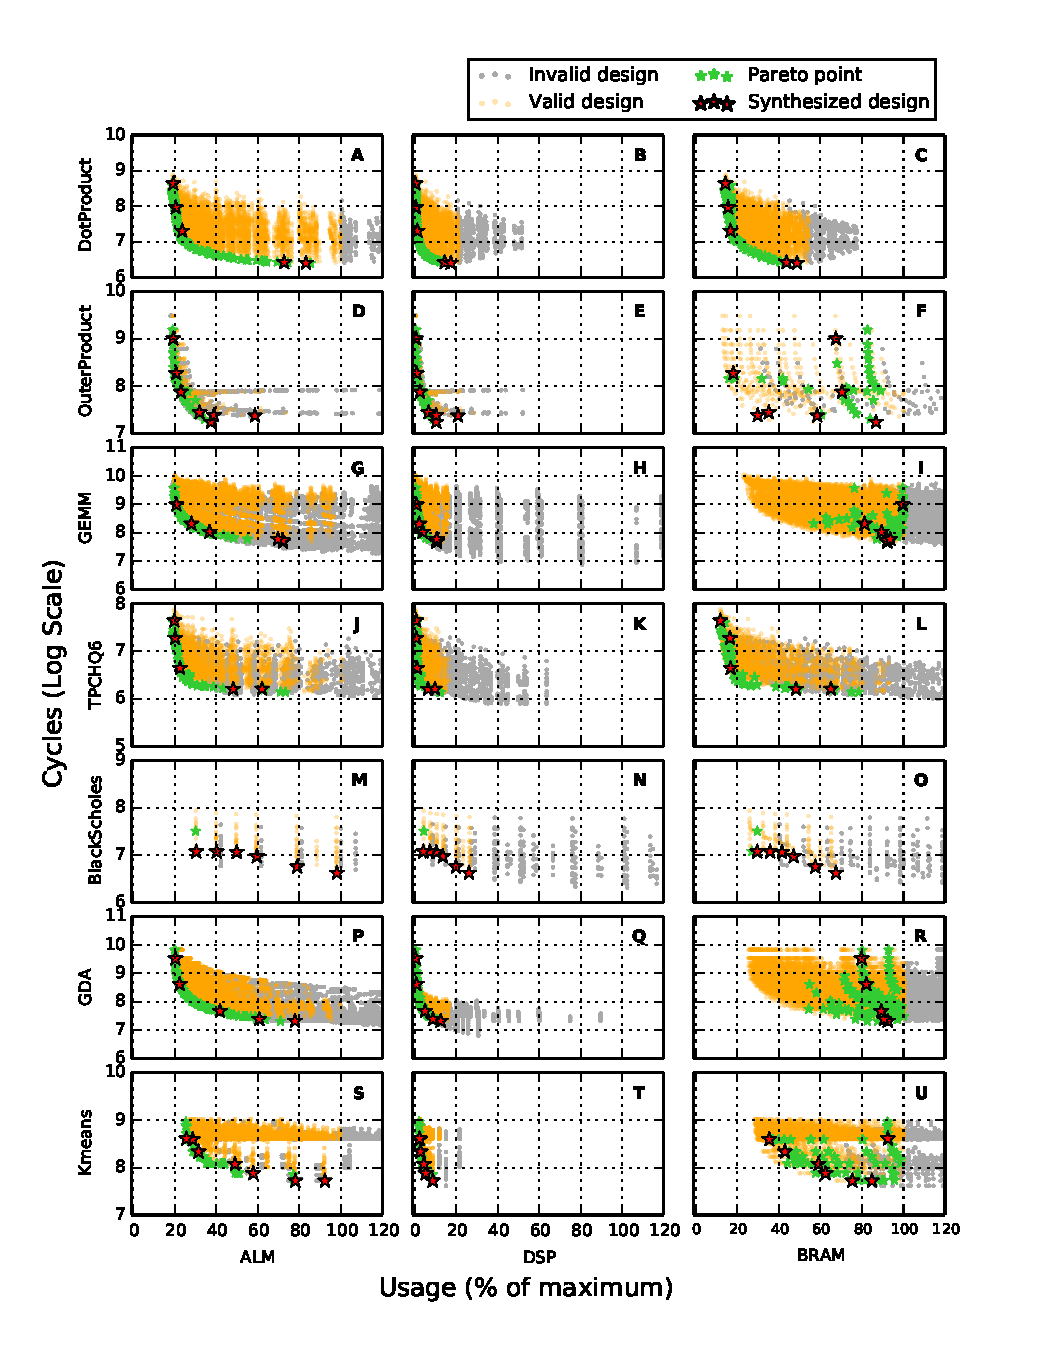
\includegraphics[width=0.95\textwidth]{figs/tradeoff.pdf}
\caption{Results of design space exploration. Horizontal axis shows estimated ALM, DSP, and BRAM usages. Vertical axis shows runtime in cycles, given in log scale (base 10).}
\label{fig:dse}
\end{figure*}

%\begin{figure*}[ht]
\subsection{Design space exploration}
\subsubsection{Pareto-optimality analysis}
In this section we show the Pareto-optimal curves of each benchmark derived from estimators.
%
Figure~\ref{fig:dse} shows the design space scatter plots for all benchmarks in
Table~\ref{t:benchmarks}. A design point is considered
invalid if its resource requirement for at least one type of resource exceeds the maximum
available amount on the target device. Pareto-optimal designs along the dimensions of execution time
and ALM utilization are highlighted for each benchmark through all three resource plots.
We now analyze each benchmark in detail.

\textbf{Dot product} (Figure~\ref{fig:dse} A,B,C) is a memory-bound benchmark. Peak execution
time is reached by balancing tile loads and computation. Inner and outer loop parallelization allows us to
quickly reach close to the input bandwidth. Runtimes of designs with \emph{MetaPipe}s then slowly decrease as parallelization
increases once the dominant stage becomes the dot product reduction tree. In \emph{dotproduct}, designs with \emph{MetaPipe} consume less resources than those with \emph{Sequential} for the same performance. \emph{Sequential}s require larger tile sizes and more parallelism to match \emph{MetaPipe} performance.

\textbf{Outer product} (Figure~\ref{fig:dse} D,E,F) represents both a BRAM and memory bound benchmark. For $2N$ inputs,
the total BRAM requirement is $2N + N^2$ to store the input and output tiles, meaning the BRAM requirement
increases quadratically with increases in input tile size. The highest performing designs for outer product do not use
\emph{MetaPipes} to overlap loading and storing of tiles. This is because the overhead due to main memory contention from overlapping
tile loads and stores turns out to be higher than the cost of executing each stage sequentially.

\textbf{GEMM} (Figure~\ref{fig:dse} G,H,I) contains a lot of temporal and spatial locality. From Figure~\ref{fig:dse}(I), Pareto-optimal designs for \emph{gemm}
occupy almost all BRAM resources on the board. Intuitively, this is  because good designs for \emph{gemm}
maximize locality by retaining large, two dimensional chunks of data in on-chip memory.
%However, as seen in Figure~\ref{fig:dse}(G), \emph{gemm} is also limited by the
%number of ALMs due to the large number of floating point operations being done in parallel.

\textbf{TPC-H Q6} (Figure~\ref{fig:dse} J,K,L) exhibits behavior typical of memory intensive applications. Performance reaches a maximum threshold
with increased tile size because of overlapping memory access and compute.

\textbf{BlackScholes} (Figure~\ref{fig:dse} M,N,O) streams through multiple large arrays and performs complex floating point computations
on the input data. Points along the same vertical bar in Figure~\ref{fig:dse}(M) share the same inner loop parallelization
factor. Increasing parallelization improves performance by increasing utilization of the available off-chip memory bandwidth.
Our model suggests that increasing the inner loop parallelization would continue to scale
performance until a parallelization of 16, around which point \emph{blackscholes} would be memory bound. Because there are not enough compute resources are available to implement a parallelization factor of 16, \emph{blackscholes} is ALM bound.

\textbf{GDA} (Figure~\ref{fig:dse} P,Q,R) possesses higher degrees of spatial locality. Because of this, \emph{gda} exhibits compute-bound behavior, where execution time
decreases steadily with increased resource utilization, as seen in Figure~\ref{fig:dse}(P). The critical resource is again BRAM. This is because BRAM usage increases with parallelization due to the creation of
more banks with fewer words per bank, which can cause under-utilization of the capacity of individual BRAMs.

\textbf{K-Means} (Figure~\ref{fig:dse} S,T,U) is bound by the number of ALMs. The critical path in this application is the distance computation done comparing an input point to each centroid.
The number of floating point operations to be done to keep up with main memory bandwidth is therefore proportional to $K \times D$, where $D$ is the number of dimensions in one point.
The performance of \emph{kmeans} is therefore limited by the number of ALMs on the FPGA, as not enough are available to perform all $K \times D$ operations in parallel.
Like GDA, \emph{kmeans} is also limited by BRAMs due to under-utilization of BRAM capacity with increased banking factors.




From our experiments, we observe that capturing parallelism at multiple levels using \emph{MetaPipe}s enables us to generate
efficient designs. In addition, effective management of on-chip BRAM resources is critical to good designs
as BRAM resources are the limiting factor for performance scaling in most of our benchmarks.
%\begin{figure*}[ht]



\subsubsection{Speed of exploration}
We compare the speed of our estimation and design space exploration with
Vivado HLS~\cite{vivadohls}, a commercial high-level synthesis tool from Xilinx.
Our evaluation uses the GDA example in Figure~\ref{fig:gda-hls} as input to the high-level synthesis tool, and the GDA
design in Figure~\ref{fig:gda-graph} as input to our design space exploration tool. Design parameters
for the high-level synthesis tool are the unrolling factors. We also include a pipeline directive
toggle for each loop in the design. For Spatial, we vary all design parameters
specified in Figure~\ref{fig:gda-code}. Speed
is measured by comparing the average estimation speed per point for 250 design points for each tool.
In our experiments, our analysis takes 5 to 29 milliseconds per design depending on the size of the application's intermediate representation.Analysis of GDA also takes 17 milliseconds per design.

\begin{table}
\centering\footnotesize
\begin{tabular}{lcc}
\toprule
{\bf Our approach}  & {\bf Vivado HLS restricted\textsuperscript{$\dagger$}} & {\bf Vivado HLS full} \\ \midrule
0.017s / design     & 4.75s / design               & 111.06s / design      \\ \midrule
\end{tabular}
\textsuperscript{$\dagger$}Vivado HLS restricted design space ignores outer loop pipelining
\caption{Average estimation time per design point.}
%The Vivado HLS design space does not include outer loop pipelining.
\label{t:speeds}
\end{table}

Table~\ref{t:speeds} shows a comparison between estimation speeds from our toolchain and Vivado HLS.
The ``restricted'' column refers to the average time spent per design over points whose outer loop ($L1$, in Figure~\ref{fig:gda-hls})
is not pipelined with a pipeline directive. The ``full'' version refers to all design points where 30 of the 250 points
have a pipeline directive to enable outer loop pipelining. We observe the following:
\begin{itemize}
  \item Our estimation tool is 279$\times$ faster than the ``restricted'' space exploration, and 6533$\times$ faster than the ``full'' space exploration.
  \item Compared to Vivado HLS, our estimation time is not sensitive to design parameter inputs. Estimation time for Vivado HLS increases
    dramatically when the outer loop is pipelined in GDA because the tool completely unrolls all inner loops
    before pipelining the outer loop. This creates a large graph that complicates scheduling. Our approach does not
    suffer from this limitation because we explicitly capture pipelines in parameterized templates such as \emph{Pipe} and
    \emph{MetaPipe}, thereby capturing outer loop pipelining more naturally.
\end{itemize}

% \begin{figure}
% \centering
% %%% trim = left, bottom, right, top
% \begin{subfigure}[t]{0.45\linewidth}
% 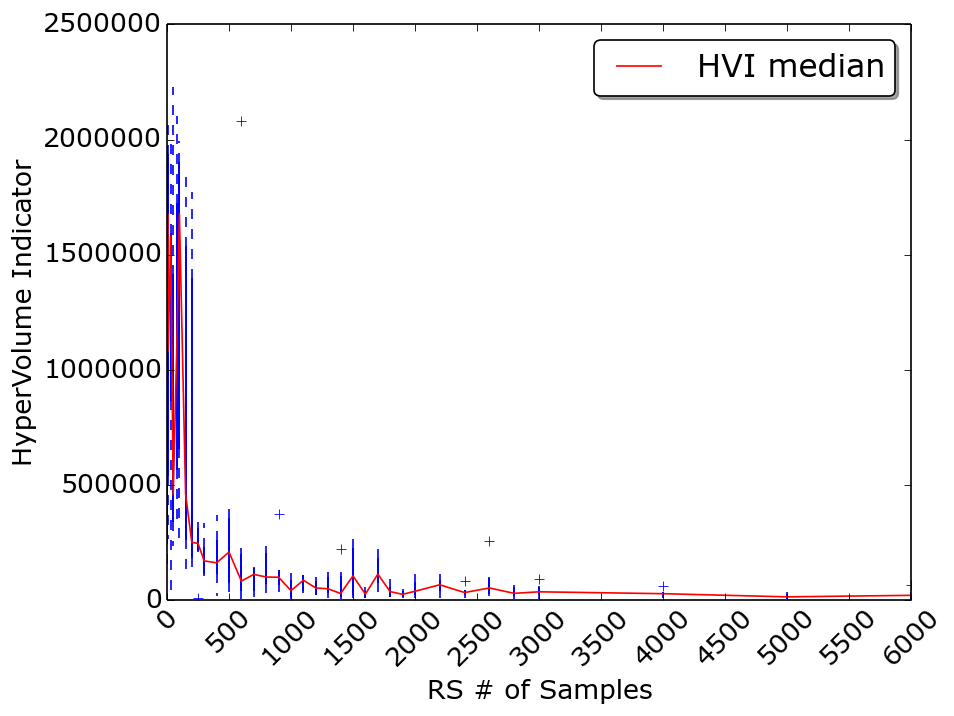
\includegraphics[width=\linewidth]{images/DSE/hvi_5NumberSummary_median.png}
% \subcaption{HyperMapper HVI versus initial random samples ($R$) five number summary.}
% \label{hvi_samples}
% \end{subfigure}\hspace{15pt}
% ~
% \begin{subfigure}[t]{0.45\linewidth}
% 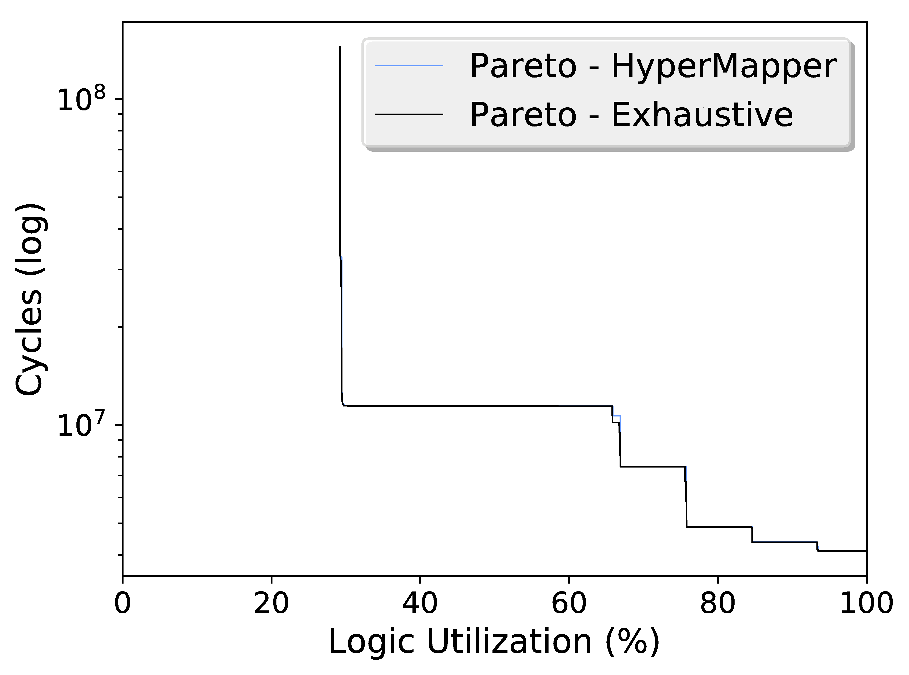
\includegraphics[clip, trim=0.0cm 0.0cm 0.0cm 0.0cm, width=\linewidth]{figs/output_pareto_blackscholes.pdf}
% \subcaption{Exhaustive and HyperMapper ($R$=1000) generated Pareto curves. }
% \label{paretos}
% \end{subfigure}
% \caption{Design space tuning on \emph{BlackScholes}.}
% \label{figHVI}
% \end{figure}

% \begin{table}[ht]
% \centering
% \caption{Runtime to reach accuracy of TODO\% and corresponding variance for design tuning with heuristic search and HyperMapper.}
% \label{tableDSE}

% \fontsize{7}{9}\selectfont
% \begin{tabular}{llrrrrr}
%                       & \multicolumn{2}{c}{\textbf{Space Size}} & \multicolumn{2}{c}{\textbf{Heuristic}} & \multicolumn{2}{c}{\textbf{HyperMapper}} \\
%                       & \mc{Total} & \mc{Pruned}    & \mc{Time} & \mc{Var}  &   \mc{Time} & \mc{Var} \\ \midrule
%   %\bf{Dot Product}   & 117,964,800      & 1,085,952            &              &                &                &               \\ \midrule
%   %\bf{Outer Product} & 16,588,800       & 31,068               &              &                &                &               \\ \midrule
%   \bf{BS}             & 7.7$\times 10^4$  & 6.7$\times 10^2$    &              &                &                &               \\ \midrule
%   \bf{GDA}            & 3.0$\times 10^{10}$ & 4.6$\times 10^6$  &              &                &                &               \\ \midrule
%   \bf{GEMM}           & 2.6$\times 10^8$  & 1.4$\times 10^5$   &              &                &                &               \\ \midrule
%   \bf{KMeans}         & 2.1$\times 10^6$  & 1.9$\times 10^4$   &              &                &                &               \\ \midrule
%   \bf{SW}             & 2.1$\times 10^6$  & 3.3$\times 10^4$   &              &                &                &               \\ \midrule
%   \bf{TQ6}            & 3.5$\times 10^9$  & 2.3$\times 10^6$   &              &                &                &               \\ \bottomrule
% \end{tabular}
% \end{table}


\subsection{Spatial Portability}

\begin{table}
\centering
\caption{Runtimes (ms) of tuned designs on ZC706, followed by runtimes and speedup~($\times$) of directly porting these designs to the VU9P, then runtimes and successive speedup over ported designs when tuned for the VU9P. The \emph{Total} column shows the cumulative speedup.}
\label{fig:zynq_comp}

\centering
\fontsize{7}{9}\selectfont
\begin{tabular}{l d{2.1} d{2.1} d{2.1} d{2.1} d{2.1} d{2.1}}
   \bf{FPGA}      & \mc{ZC706}  & \multicolumn{4}{c}{\bf VU9P}                                       & \mc{Total}     \\
   \bf{Design}    & \mc{Tuned}  & \multicolumn{2}{c}{\bf Ported}   & \multicolumn{2}{c}{\bf Tuned}    &               \\ \toprule

                  & \mc{Time}   & \mc{Time}  & \mc{$\times$}       & \mc{Time}  & \mc{$\times$}       & \mc{$\times$} \\ \midrule
   \ml{BS}        & 89.0        & 35.6       & 2.5                 & 3.8        & 9.4                 & 23.4          \\ \midrule
   \ml{GDA}       &  8.4        & 3.4        & 2.5                 & 1.3        & 2.6                 & 6.5           \\ \midrule
   \ml{GEMM}      & 2226.5      & 1832.6     & 1.2                 & 878.5      & 2.1                 & 2.5           \\ \midrule
   \ml{KMeans}    & 358.4       & 143.4      & 2.5                 & 53.3       & 2.7                 & 6.7           \\ \midrule
   \ml{PageRank}  & 1299.5      & 1003.3     & 1.3                 & 587.4      & 1.7                 & 2.2           \\ \midrule
   \ml{SW$^\dag$} & 1.3         &  0.5       & 2.5                 & 0.5        & 1.0                 & 2.5           \\ \midrule
   \ml{TQ6}       & 69.4        & 15.0       & 4.6                 & 14.0       & 1.1                 & 5.0           \\ \bottomrule

   \multicolumn{7}{l}{\vspace{10pt}\footnotesize{ $^\dag$SW with 160 base pairs, the largest to fit on the ZC706.}}
\end{tabular}
\end{table}

We next demonstrate the portability of Spatial code by targeting two different FPGA architectures; (1) the Zynq ZC706 SoC board, and (2) The Virtex Ultrascale+ VU9P on the Amazon EC2 F1.
Designs on the VU9P use a single DRAM channel with a peak bandwidth of 19.2 GB/s. The ZC706 is much smaller than the VU9P in terms of FPGA resource and has a smaller DRAM bandwidth of 4.26 GB/s.
We target both the ZC706 and VU9P from the same Spatial code for all benchmarks listed in Table~\ref{t:hls_comp}. Benchmarks are tuned for each target using
target-specific models with automated DSE. Clock frequency is fixed at 125 MHz for both FPGAs.

Table~\ref{fig:zynq_comp} shows the speedups achieved on the VU9P over the ZC706. The results show that not only can the same Spatial source code be ported
to architectures with different capabilities, the application can also be automatically tuned to better take advantage of resources in each target.
Compute-bound benchmarks \emph{BlackScholes}, \emph{GDA}, \emph{GEMM}, \emph{K-Means} achieve speedups of up to $23\times$ on the VU9P over the ZC706. Porting these designs to the VU9P alone has a $1.2\times$ to $2.5\times$ due to increased main memory bandwidth, but a majority of the benefit of the larger FPGA comes from tuning the parallelization factors to use more resources.
While \emph{SW} is also compute bound, the size of the dataset was limited by the smaller FPGA. In this case, the larger capacity of the VU9P does not improve runtime, but instead allows handling of larger datasets.

Memory-bound benchmark \emph{TPC-H Q6} benefits from the higher DRAM bandwidth available on the VU9P. Porting this benchmark immediately gives a $4.6\times$ runtime improvement from the larger main memory bandwidth, while further parallelizing controllers to create more parallel address streams to DRAM helps the application make better use of this bandwidth. \emph{PageRank} is also bandwidth-bound, but the primary benefit on the VU9P comes from specializing the memory controller to maximize utilized bandwidth for sparse accesses.


% \begin{table}
% \caption{Speedup of VU9P over ZC706.}
% \label{fig:zynq_comp}

% \fontsize{8}{10}\selectfont
% \begin{tabular}{cccccc}
% \bf{GDA}     & \bf{GEMM}    & \bf{K-Means} & \bf{PageRank} & \bf{SW}      & \bf{TQ6} \\ \hline
% 2.54$\times$ & 2.53$\times$ & 1.84$\times$ & 2.21$\times$  & 1.74$\times$ & 4.97$\times$  \\ \hline
% \end{tabular}
% \end{table}




\begin{table}
\centering
\caption{Plasticine DRAM bandwidth, resource utilization, runtime, and speedup ($\times$) over VU9P FPGA.}
\label{table:plasticine_eval}
\centering
\fontsize{7}{7}\selectfont
\resizebox{0.99\columnwidth}{!}{
  \begin{tabular}{m{0.5cm} d{2.1} d{2.1} d{2.1} d{2.1} d{2.1} d{2.1} r }
  \toprule
                 & \multicolumn{2}{c}{\bf Avg DRAM } & \multicolumn{3}{c}{\bf Resource }        & \mc{}     & \mc{} \\
                 & \multicolumn{2}{c}{\bf BW (\%)}   & \multicolumn{3}{c}{\bf Utilization (\%)} & \mc{Time} & \mc{$\times$} \\
   \bf{App}     & \mc{Load}    & \mc{Store} & \mc{PCU}  & \mc{PMU}  & \mc{AG}   & \mc{(ms)} & \mc{} \\ \midrule
   \ml{BS}       & 77.4        & 12.9       & \mb{\hspace{1pt}73.4} & 10.9      & 20.6      & 2.33      & 1.6   \\
   \ml{GDA}      & 24.0        & 0.2        & \mb{\hspace{1pt}95.3} & 73.4      & 38.2      & 0.13      & 9.8   \\
   \ml{GEMM}     & 20.5        & 2.1        & \mb{\hspace{1pt}96.8} & 64.1      & 11.7      & 15.98     & 55.0  \\
   \ml{KMeans}   & 8.0         & 0.4        & \mb{\hspace{1pt}89.1} & 57.8      & 17.6      & 8.39      & 6.3   \\
   \ml{TQ6}      & \mb{\hspace{2pt}97.2}   & 0.0        & 29.7      & 37.5      & \mb{70.6} & 8.60      & 1.6   \\

\bottomrule
\end{tabular}}
\end{table}


Finally, we demonstrate the portability of Spatial beyond
FPGA architectures by extending the compiler to map
the Spatial IR to target our proposed Plasticine CGRA~\cite{plasticine}. Plasticine is a
two-dimensional array of compute (PCUs) and memory
(PMUs) tiles with a statically configurable interconnect
and address generators (AG) at the periphery to perform
DRAM accesses. The Plasticine architecture is a significant departure
from an FPGA, with more constraints on memory banking and computation, including
fixed size, pipelined SIMD lanes.

We simulate Plasticine with  a $16 \times 8$ array of 64 compute and 64 memory tiles, with a 1 GHz clock and a main memory with a DDR3-1600 channel with 12.8 GB/s peak bandwidth.
Table~\ref{table:plasticine_eval} shows the DRAM bandwidth, resource utilization, runtime, and speedup of the Plasticine CGRA over the VU9P for a subset of benchmarks.

Streaming, bandwidth-bound applications like \emph{TPC-H Q6} efficiently exploit about 97\% of the available DRAM bandwidth.
Compute-bound applications \emph{GDA}, \emph{GEMM}, and \emph{K-Means} use around 90\% of Plasticine's compute tiles.
Plasticine's higher on-chip bandwidth also allows these applications to better utilize the compute resources, giving these applications speedups of $9.9\times$, $55.0\times$, and $6.3\times$.
Similarly, the deep compute pipeline in \emph{BlackScholes} occupies 73.4\% of compute resources after being split across multiple tiles,
giving a speedup of $1.6\times$.

%We implemented comparable versions of each of our benchmarks in C++ and synthesized them
%using HLS and SDAccel tools.  There are certain constructs in Spatial that allow
%certain algorithms to be expressed more concisely and in slightly different, but intuitive, ways that
%expose the strengths of the language.  Each application exhibits certain characteristics which
%can be exploited by certain aspects in the programming paradigms of Spatial and HLS. Specifically,
%they can be characterized as compute-bound applications and memory-bound applications, with some
%tradeoff between the two depending on design decisions.  While HLS is the industry standard for
%exposing FPGAs to domain experts, our results show that Spatial is a suitable alternative that can
%lead to better designs for certain algorithms with less overhead.

%Spatial is a suitable platform for the designer who is interested in making the most of the
%available resources, as it allows quick design tradeoffs in the app without needing to use complex pragmas throughout the app.
%In applications that are memory bound, such as AES, BlackScholes, and Sobel, we would expect that neither
%design could acheive significantly better speedup since they have access to the same DRAM interfaces.
%For compute-bound applications, such as Kmeans, GEMM, and GDA, there is a large, interesting design space that
%Spatial can quickly expose to the user.

%\begin{figure}
%\centering
%\includegraphics[width=1\columnwidth, trim=0.5cm 0.9cm 1.0cm 0]{figs/f1_comp.png}
%\caption{Speedup and resource utilization comparisons with SDAccel on F1.}
%\label{fig:f1_comp}
%\end{figure}

% \subsection{Portability Across FPGAs and CGRAs}
% We demonstrate the applicability of Spatial to beyond FPGA architectures by extending the compiler
% to map Spatial IR to the Plasticine CGRA~\cite{plasticine}. Plasticine is a two-dimensional array of compute (PCUs) and memory (PMUs) tiles
% with a statically configurable interconnect and address generators (AG) at the periphery to perform DRAM accesses.
% Plasticine is a significant departure from FPGA with different kinds of constraints on memory banking and parallelization.

% Similar to the FPGA, we construct area and runtime models specific to Plasticine, and drive the design space exploration to tune
% benchmarks to Plasticine. Compiling to Plasticine then involves lowering the Spatial IR to a target-specific IR for the Plasticine low-level mapping compiler,
% which outputs a configuration bitstream. Resource utilization reports are obtained from the low-level compiler.
% Execution times are measured by simulating the generated bitstream in a cycle-accurate fashion at a clock frequency of 1 GHz.



%Fortunately, due to the locality exhibited by these applications, designs with large tile sizes that do not maximize the off-chip
%bandwidth are capable of achieving comparable performance to the ones that have 100\%
%compute unit utilization. Hence, the best performing design point shown in
%Table~\ref{table:plasticine_eval} does not correspond to the design with 100\% compute utilization.

%Therefore, the given architecture cannot fit unrolling the outer loop by more than 1 without
%exceeding 100\% PCU utilization.
%\todo{K-Means is a sequential iterative convergence algorithm that neither outer loop nor
%inner loop that computes the new centroids can be parallelized.} As a result, we could not maximize
%either bandwidth or resource.}

%For application that are not memory-bound, yet Plasticine is not able to take larger
%unrolling factors, such as BlackScholes and K-Means, Plasticine still achieves roughly $4-7\times$
%speedup compared to F1 due to its higher clock frequency.

%Figure~\ref{fig:gemm_dse} shows the design space of GEMM on Plasticine. The bottom edged circles are
%designs with large tile size that better capture locality. The dark large circles on the right are
%designs with good PCU and PMU utilization, and high DRAM load bandwidth as result of outer loop
%unrolling.



%\begin{figure}
%\centering
%\includegraphics[width=1\columnwidth]{figs/GEMM_Blocked.png}
%\caption{Design space for GEMM on Plasticine}
%\label{fig:gemm_dse}
%\end{figure}

%\begin{figure}
%\centering
%\begin{minipage}{.5\linewidth}
  %\centering
  %\includegraphics[width=1\linewidth]{reg_K-FOLD}
  %\caption{Regularization}
  %\label{fig:reg}
%\end{minipage}%
%\end{figure}
%\subsection{GEMM Case Study}
%\gist{gemm}

\section{Conclusion}
\todo{Conclusion!}

